\documentclass[../notes.tex]{subfiles}

\pagestyle{main}
\renewcommand{\chaptermark}[1]{\markboth{\chaptername\ \thechapter\ (#1)}{}}
\stepcounter{chapter}

\begin{document}




\chapter{Bonding Models}
\section{Bonding Models 1}
\begin{itemize}
    \item \marginnote{9/10:}Lecture 1 recap.
    \begin{itemize}
        \item Aspects of mechanism.
        \begin{itemize}
            \item Orbitals, energy surface, and kinetics.
            \item Masha redraws Figure \ref{fig:mechAspects}.
            \item These are the three main pictures that we'll learn about.
        \end{itemize}
        \item Today, we'll focus on orbitals.
    \end{itemize}
    \item Today: Bonding models.
    \begin{itemize}
        \item Reading: \textcite{bib:Anslyn}, Chapter 1!!
    \end{itemize}
    \item \textbf{Bonding}: How electrons are shared between nuclei.
    \begin{itemize}
        \item This determines all of molecular structure and reactivity (which is the name of this class, and underpins all of organic chemistry!).
        \item From bonding, there arise concepts such as nucleophilicity, electrophilicity, etc.
    \end{itemize}
    \item There are several levels of bonding theory / models that we'll talk about today.
    \begin{itemize}
        \item Caveat: \emph{All} of these models are no more than \emph{approximations} of reality that are useful to us.
    \end{itemize}
    \item Lecture outline.
    \begin{enumerate}
        \item Lewis structures.
        \item VSEPR.
        \item Valence Bond Theory (VBT).
        \item Molecular Orbital Theory.
        \item Qualitative Molecular Orbital Theory (QMOT).
    \end{enumerate}
    \item Lewis structures.
    \begin{figure}[h!]
        \centering
        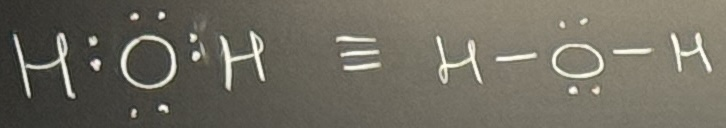
\includegraphics[width=0.2\linewidth]{LewisDots.JPG}
        \caption{Lewis dot structures.}
        \label{fig:LewisDots}
    \end{figure}
    \pagebreak
    \begin{itemize}
        \item Developed in 1916 by G. N. Lewis.
        \begin{itemize}
            \item Chemis-tea: He was nominated 48 times, but never won the Nobel Prize because some people on the review committee didn't like his "interesting personality."
        \end{itemize}
        \item In this model, we use dots to --- on paper --- indicate where electrons are in bonds.
        \item From these \textbf{Lewis dot structures}, people developed the "stick structures" that we still use today.
        \item Lewis structures are very useful in identifying the number of bonds and lone pairs.
    \end{itemize}
    \item Valence Shell Electron Pair Repulsion (VSEPR).
    \begin{itemize}
        \item Developed 1939-1957.
        \item Key finding: Electrons in bonds repel each other, so you maximize the distance between bonds.
        \item This let us go beyond Lewis structures into things like explaining tetrahedral carbon (and its \ang{109.5} bond angles).
        \item Issues develop when we try to rationalize other molecules.
        \begin{itemize}
            \item For example, isobutane has \ang{110.6} \ce{Me-C-Me} bond angles. The VSEPR purists will cite "sterics."
            \item As another example, \ce{NH3} has \ce{107} \ce{H-N-H} bond angle. The VSEPR purists will cite "lone pair is big."
        \end{itemize}
        \item Really, these were just excuses by the VSEPR purists for a bad model, and what we really needed was a new model.
    \end{itemize}
    \item Valence Bond Theory (VBT).
    \begin{itemize}
        \item Developed by Linus Pauling, with his seminal paper in 1931.
        \begin{itemize}
            \item For this work and some other stuff, he won the Nobel Prize in Chemistry in 1954.
            \item To be historically accurate, Pauling built off the work of Heitler and London (1926).
            \item However, Pauling was the person to both put everybody else's work all together and be visible enough to take the credit.
            \item Additional takeaway from Pauling's biography: Don't make your whole life about your work. For example, Pauling was shunned by many of his colleagues after he got into nuclear proliferation, but now we say he was so brave. He even won the Nobel Peace Prize!
            \item Takeaway on Pauling vs. Lewis: It pays to not be a jerk. Lewis died via cyanide poisoning (may have been an accident, but was probably suicide).
        \end{itemize}
        \item This is a quantum mechanical (QM) description of Lewis structures.
        \item Central tenet: Each atom contributes 1 valence electron in a QM-derived atomic orbital (AO).
        \begin{itemize}
            \item Shows that electrons are delocalized between atoms, and where two electrons overlap and localize is a chemical bond.
            \item In other words, electrons are not restricted to tight orbitals.
        \end{itemize}
        \item Many concepts arise within VBT until the advent of MO theory.
    \end{itemize}
    \item VBT was key for many conceptual innovations, such as \textbf{hybridization}, \textbf{electronegativity}, and \textbf{resonance}.
    \item \textbf{Hybridization}: The mixing of orbitals on the same atom to make new orbitals.
    \begin{itemize}
        \item Specifically, we can take a linear combination of AO waveforms (or AOs).
        \item More directional orbitals give you better overlap and therefore stronger bonds.
        \item Example: A linear combination $s+p_y+p_x+p_z$ yields four $sp^3$-hybridized orbitals. That's four orbitals with uneven lobes. We can draw all of these on top of each other, and from \emph{there}, we get the tetrahedral carbon.
        \item We always like new models that agree with old models; this is called a \textbf{sanity check}.
        \item We can also calculate something called the \textbf{hybridization index}.
    \end{itemize}
    \item \textbf{Hybridization index}: The number $i$ in the following formula, expressed as a function of the experimentally determined bond angle $\theta$. \emph{Denoted by} $\bm{i}$. \emph{Given by}
    \begin{equation*}
        1+i\cos\theta = 0
    \end{equation*}
    \begin{itemize}
        \item Example: \ce{NH3} has a hybridization index of 3.4.
        \item Example: \ce{H2O} has a hybridization index of 4! That's why it has the tiny bond angle. The remaining $s$-character is localized on the oxygen, and that's why we say that oxygen is electron dense and nucleophilic.
        \begin{itemize}
            \item Would this similarly predict that \ce{H2O} has longer bonds than \ce{NH3}??
        \end{itemize}
    \end{itemize}
    \item \textbf{Electronegativity}: The power of an atom to attract electrons to itself.
    \begin{itemize}
        \item There are different scales for this. We probably used the \textbf{Pauling scale}, but there is also a \textbf{Mulliken scale}.
        \item More electronegative atoms have lower energy orbitals.
        \begin{itemize}
            \item This is summarized via the \textbf{inductive effect}.
        \end{itemize}
    \end{itemize}
    \item \textbf{Inductive effect}: The withdrawing of electron density through $\sigma$-bonds.
    \begin{itemize}
        \item Example: ACN. We think about nitrogen having a partial negative charge and carbon having a partial positive charge. This results in a dipole.
        \item Takeaway: Dipoles arise from electronegativity in VBT!
    \end{itemize}
    \item \textbf{Resonance}: The superposition of several Lewis structures. \emph{Antiquated} \textbf{mesomerism}.
    \begin{itemize}
        \item Example: Consider an $\alpha,\beta$-unsaturated ketone. Its resonance structure is a zwitterionic intermediate, and a second resonance structure is a different zwitterion. We have three resonance forms, so that predicts more stable than something with less resonance structures. It also identifies our positive and negative reactive sites.
        \item Resonance usually happens through $\pi$-networks, but it \emph{can} happen through $\sigma$-networks.
        \item Takeaway: Delocalization of electron density leads to stability.
        \item Know your rules for drawing good resonance structures.
        \begin{itemize}
            \item We only move bonds, not atoms (no nuclear motion).
            \item Prefer to have the least separation of charge.
            \item Put the more negative charge on the more electronegative atoms.
        \end{itemize}
    \end{itemize}
    \item Limitations of VBT.
    \begin{itemize}
        \item Over time, some key experimental findings emerged that VBT coudn't explain. These results motivated people to develop a new model to explain these rare cases.
        \begin{itemize}
            \item Nowadays, exceptions to VBT are not so rare.
        \end{itemize}
        \item Remember: If a model can't explain certain cases, it's not a useful model.
        \begin{itemize}
            \item Maxim: Not predictive = not useful.
        \end{itemize}
    \end{itemize}
    \item Here's a list of the limitations of VBT.
    \begin{itemize}
        \item Doesn't account for unusual stability/instability (e.g., aromaticity and antiaromaticity).
        \item No antibonding orbitals (i.e., no explanation of interactions between molecules).
        \begin{itemize}
            \item When a nucleophile attacks a ketone, the interaction is with the antibonding orbital of the ketone. Forming a new bond involves populating an antibonding orbital.
        \end{itemize}
        \item Thursday is all about aromaticity, and modern ways to conceptualize it.
    \end{itemize}
    \pagebreak
    \item This leads to the mother of all bonding models, Molecular Orbital Theory.
    \begin{itemize}
        \item Central tenet: Molecular orbitals (e.g., $\sigma$, $\sigma^*$, $\pi$, $\pi^*$) arise from linear combinations of atomic orbitals (in Orgo, this is $s$ \& $p$; we won't consider $d$-orbital effects so much).
        \item We consider the electronic structure of the whole molecule, not just atoms or bonds.
        \begin{itemize}
            \item We focus on key molecular orbitals such as the HOMO and LUMO.
        \end{itemize}
        \item We also get \textbf{group orbitals}: Leads into QMOT, which is MOs for prototypical groups.
    \end{itemize}
    \item MO theory leads to MO diagrams.
    \begin{figure}[h!]
        \centering
        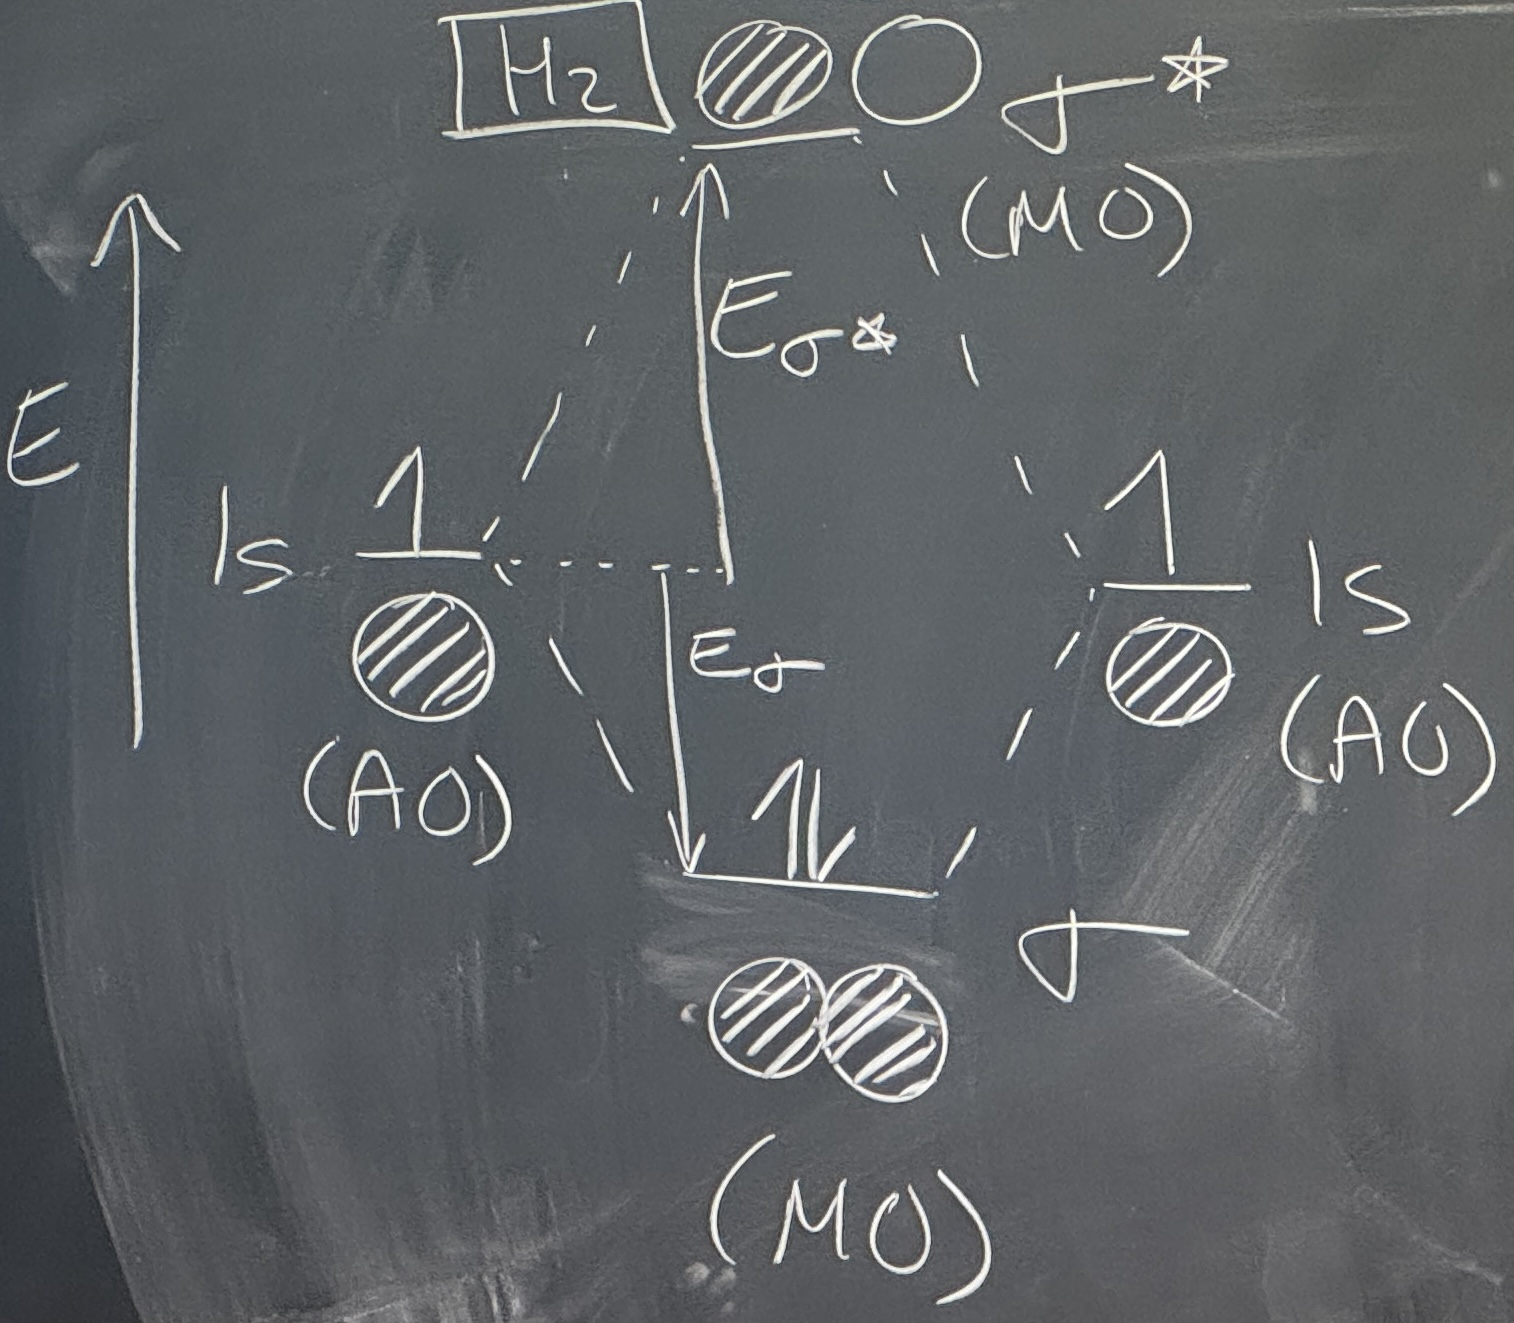
\includegraphics[width=0.3\linewidth]{MOH2.JPG}
        \caption{MO diagram for \ce{H2}.}
        \label{fig:MOH2}
    \end{figure}
    \begin{itemize}
        \item Two atomic orbitals interact to fill two molecular orbitals.
        \item We fill the bonding orbital with all the electrons that come in (in this case, 2).
        \item The energy of stabilization is $E_{\sigma}$.
        \item The destabilization energy is $E_{\sigma^*}$.
        \item Read \textcite{bib:Anslyn} for more rules.
        \item Notes.
        \begin{itemize}
            \item $|E_{\sigma^*}|>|E_{\sigma}|$. Thus, if the antibonding orbitals get populated, the moleucle breaks. This is because of nuclear repulsion.
            \item The $\sigma$-bond is more stable than the $1s$ orbitals by themselves. This is why the \ce{H-H} bond forms. This kind of analysis allows us to predict whether or not a bond will form.
        \end{itemize}
        \item Question for us to consider: Why doesn't \ce{He-He} form?
        \begin{itemize}
            \item Because its antibonding MOs would be populated.
        \end{itemize}
    \end{itemize}
    \item Example MO diagram: Ethylene.
    \begin{figure}[H]
        \centering
        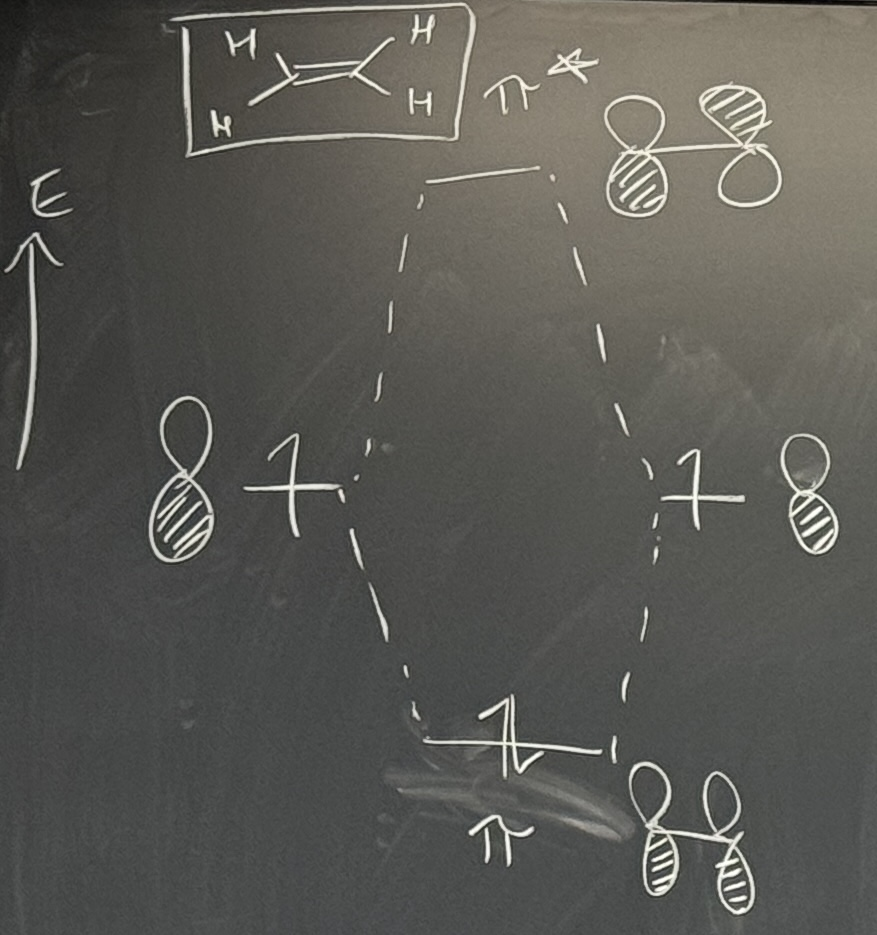
\includegraphics[width=0.3\linewidth]{MOEtH.JPG}
        \caption{MO diagram for ethylene.}
        \label{fig:MOEtH}
    \end{figure}
    \begin{itemize}
        \item Looking specifically at the $\pi$-bond formation.
        \item This is why we form a stable $\pi$-bond.
    \end{itemize}
    \item Example MO diagram: Formaldehyde.
    \begin{figure}[h!]
        \centering
        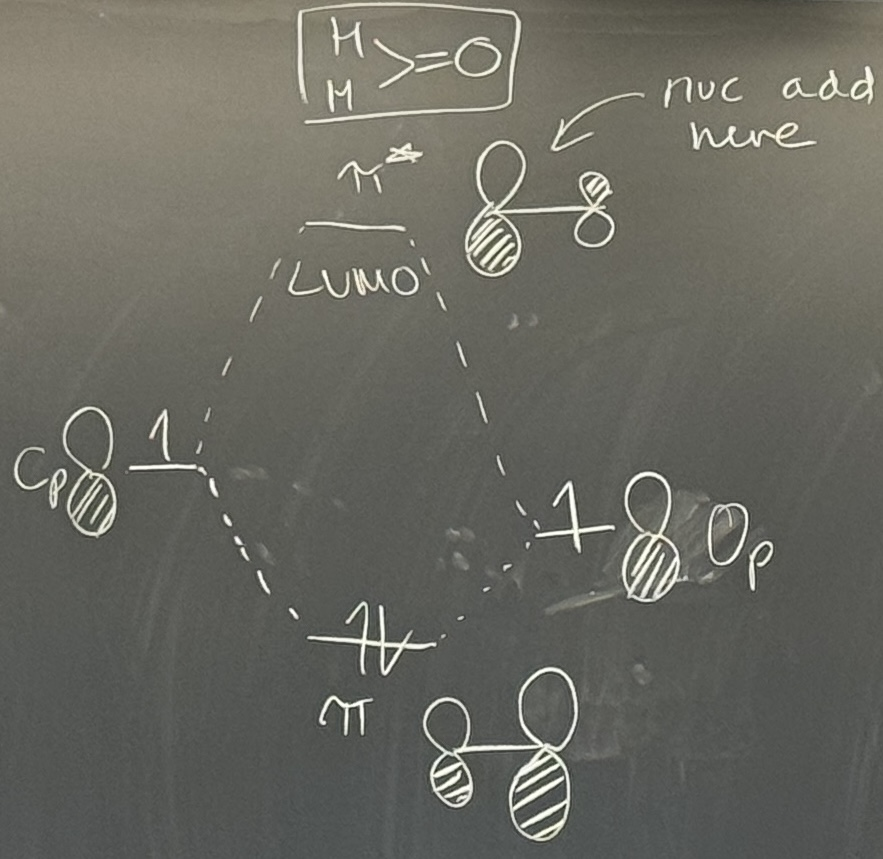
\includegraphics[width=0.3\linewidth]{MOForm.JPG}
        \caption{MO diagram for formaldehyde.}
        \label{fig:MOForm}
    \end{figure}
    \begin{itemize}
        \item We mix a \ce{C_{$p$}} AO and a (lower energy) \ce{O_{$p$}} AO.
        \item These orbitals interact less well than those in ethylene due to their difference in energy.
        \item We benefit from constructive phasing, but the lobes are much bigger on oxygen.
        \item In the antibonding orbital, the lobes are much bigger on carbon.
        \item Principles revealed by this MO diagram.
        \begin{itemize}
            \item Closer energy AOs give stronger mixing, resulting in lower energy MOs. Lower energy MOs are more stabilizing.
            \item More electronegative atoms have lower energy atomic orbitals.
            \item The $\pi$-orbital is asymmetric because its energetically more similar to \ce{O_{$p$}} than \ce{C_{$p$}}.
            \begin{itemize}
                \item In other words, it's going to look more like the \ce{O_{$p$}} orbital.
                \item One more way of stating this is that the coefficient of oxygen in the LCAO is bigger.
            \end{itemize}
        \end{itemize}
        \item We know that the LUMO (frontier orbital) interacts with nucleophiles. The lobe of the LUMO is bigger on carbon, hence why we react there.
    \end{itemize}
    \item Qualitative MO theory (QMOT).
    \begin{itemize}
        \item All about forming group orbitals for common functional groups or motifs.
        \item Essentially, we may not need to calculate MOs for the whole molecule to find out how every carbonyl reacts; we can trust that carbonyl group orbitals are decently conserved.
        \item There are a bunch of rules for how to form a QMOT diagram.
        \begin{itemize}
            \item See Table 1.7 in \textcite{bib:Anslyn} for building QMOT diagrams.
        \end{itemize}
        \item This is the basis of \textbf{Walsh diagrams}.
        \item We can build group MOs from linear combinations of $s$ \& $p$ AOs.
    \end{itemize}
    \item \textbf{Walsh diagram}: A representation of an MO diagram as a function of geometric distortions.
    \begin{itemize}
        \item This matters because geometry affects orbital overlap, which can be destabilizing or stabilizing.
    \end{itemize}
    \pagebreak
    \item Example QMOT diagram: \ce{CH3}.
    \begin{figure}[h!]
        \centering
        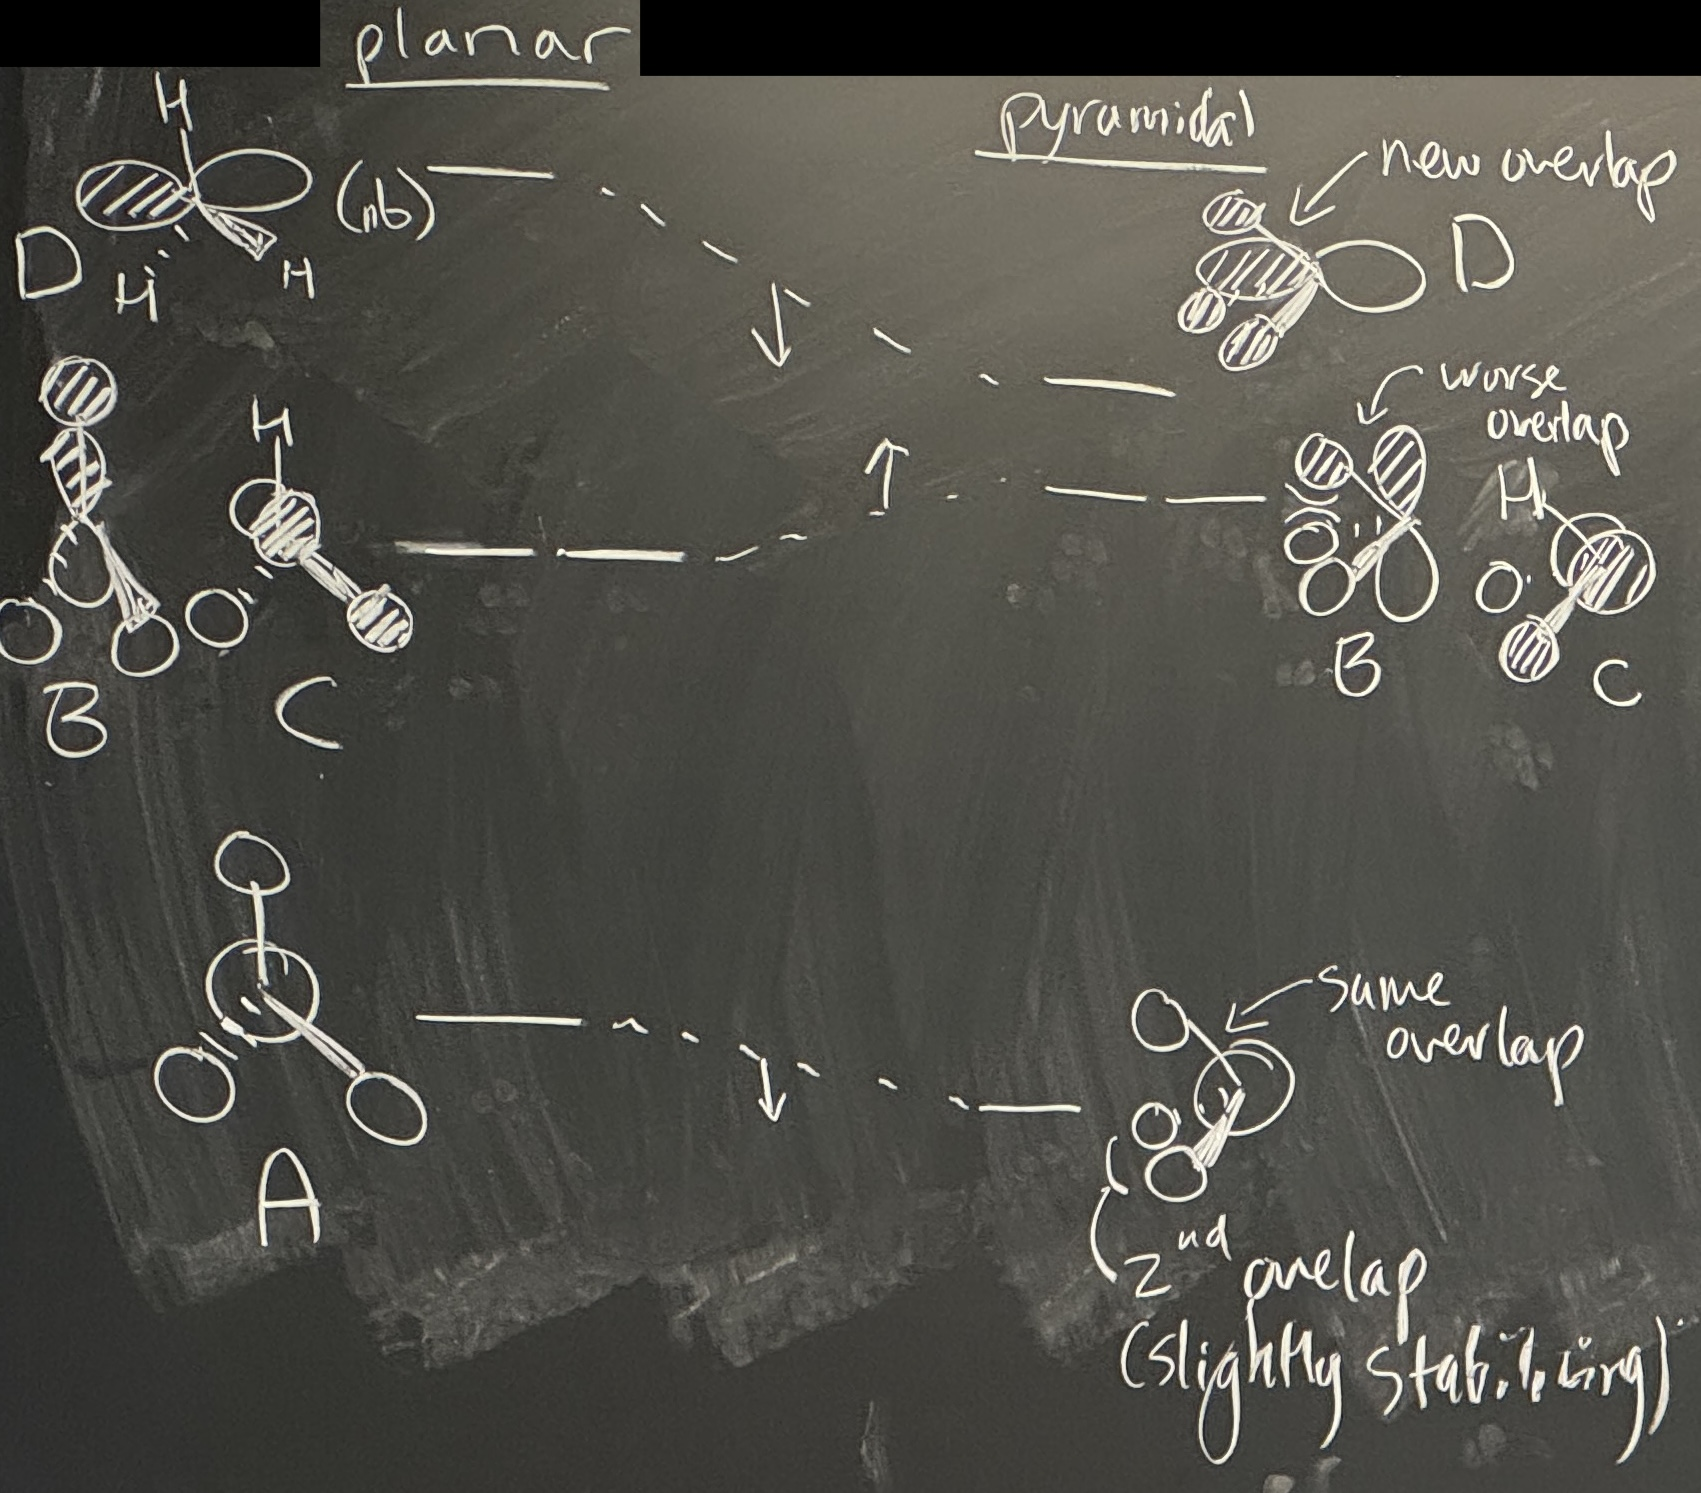
\includegraphics[width=0.4\linewidth]{QmotCH3.JPG}
        \caption{QMOT diagram for \ce{CH3}.}
        \label{fig:QmotCH3}
    \end{figure}
    \begin{itemize}
        \item Key question: What geometry of \ce{CH3} is favorable?
        \item Masha defines axes.
        \item Undetermined yet if this is a radical, cation, or anion. We'll get there!
        \item We look at a planar set of orbitals first.
        \begin{enumerate}[label={\textbf{\Alph*}.}]
            \item All phases in sync, all $s$ orbitals.
            \item Phases align top to bottom with the $p_x$ orbital of carbon.
            \item Phases align in and out of the board with the $p_y$ orbital of carbon.
            \item Nonbonding; just the $p_z$ orbital.
        \end{enumerate}
        \item There are also \textbf{E}, \textbf{F}, and \textbf{G} orbitals that are energetically above these, but we won't draw them for now (because we won't fill them with electrons in the carbocation, carbanion, or carbon radical).
        \begin{itemize}
            \item The \textbf{E}, \textbf{F}, and \textbf{G} orbitals will have the opposite phasing of the lower orbitals!
        \end{itemize}
        \item We now draw an analogous, pyramidal set of orbitals.
        \begin{enumerate}[label={\textbf{\Alph*}.}]
            \item Overlap is \emph{slightly} more favorable because we have a secondary orbital interaction between the hydrogens now. The \ce{C-H} overlap stays the same.
            \item Worse overlap. We're losing a \textbf{primary} interaction instead of gaining a \textbf{secondary} one, so the energy of \textbf{B} actually goes up \emph{more} than \textbf{A} went down. We also get some destabilizing secondary interaction between the \ce{H} orbitals.
            \item Just like \textbf{B}, we get worse primary overlap, and new interfering secondary overlap.
            \item Gets stabilized the \emph{most} significantly! This is because we've taken something with no bonding interactions and \emph{created} bonding interactions between the $p$-orbital and the hydrogens.
        \end{enumerate}
        \item Relationship between QMOT and Walsh diagrams: A Walsh diagram is a QMOT diagram with everything connected.
        \item Now how do we fill electrons?
        \begin{itemize}
            \item Consider the \ce{CH3+} cation: We have 6 electrons, so we populate the planar orbitals because it's more stable overall.
            \item Consider the \ce{CH3-} anion: We have 8 electrons, so we populate the pyramidal orbitals because \emph{they're} more stable overall.
        \end{itemize}
        \item This rigorous prediction of conformation is the benefit of this model.
        \item We can also use this model for other isostructural molecules.
        \pagebreak
        \item Examples.
        \begin{itemize}
            \item \ce{NH3}: 8 electrons, pyramidal.
            \item \ce{BH3}: 6 electrons, planar.
            \item \ce{*CH3}: 7 electrons, \emph{slightly} planar.
            \begin{itemize}
                \item But this is a special case only for \ce{*CH3}; any other radical is pyramidal.
            \end{itemize}
        \end{itemize}
    \end{itemize}
    \item \textbf{Primary} (orbital interaction): An interaction between orbitals on adjacent atoms in a molecule.
    \item \textbf{Secondary} (orbital interaction): An interaction between orbitals on atoms that are separated by one other atom in a molecule.
    \item What is quantitative about QMOT?
    \begin{itemize}
        \item There is a lot more depth in \textcite{bib:Anslyn}. You can calculate the actual potential energy surface and figure out these conformations exactly.
    \end{itemize}
    \item Example QMOT diagram: \ce{CH2}.
    \begin{figure}[h!]
        \centering
        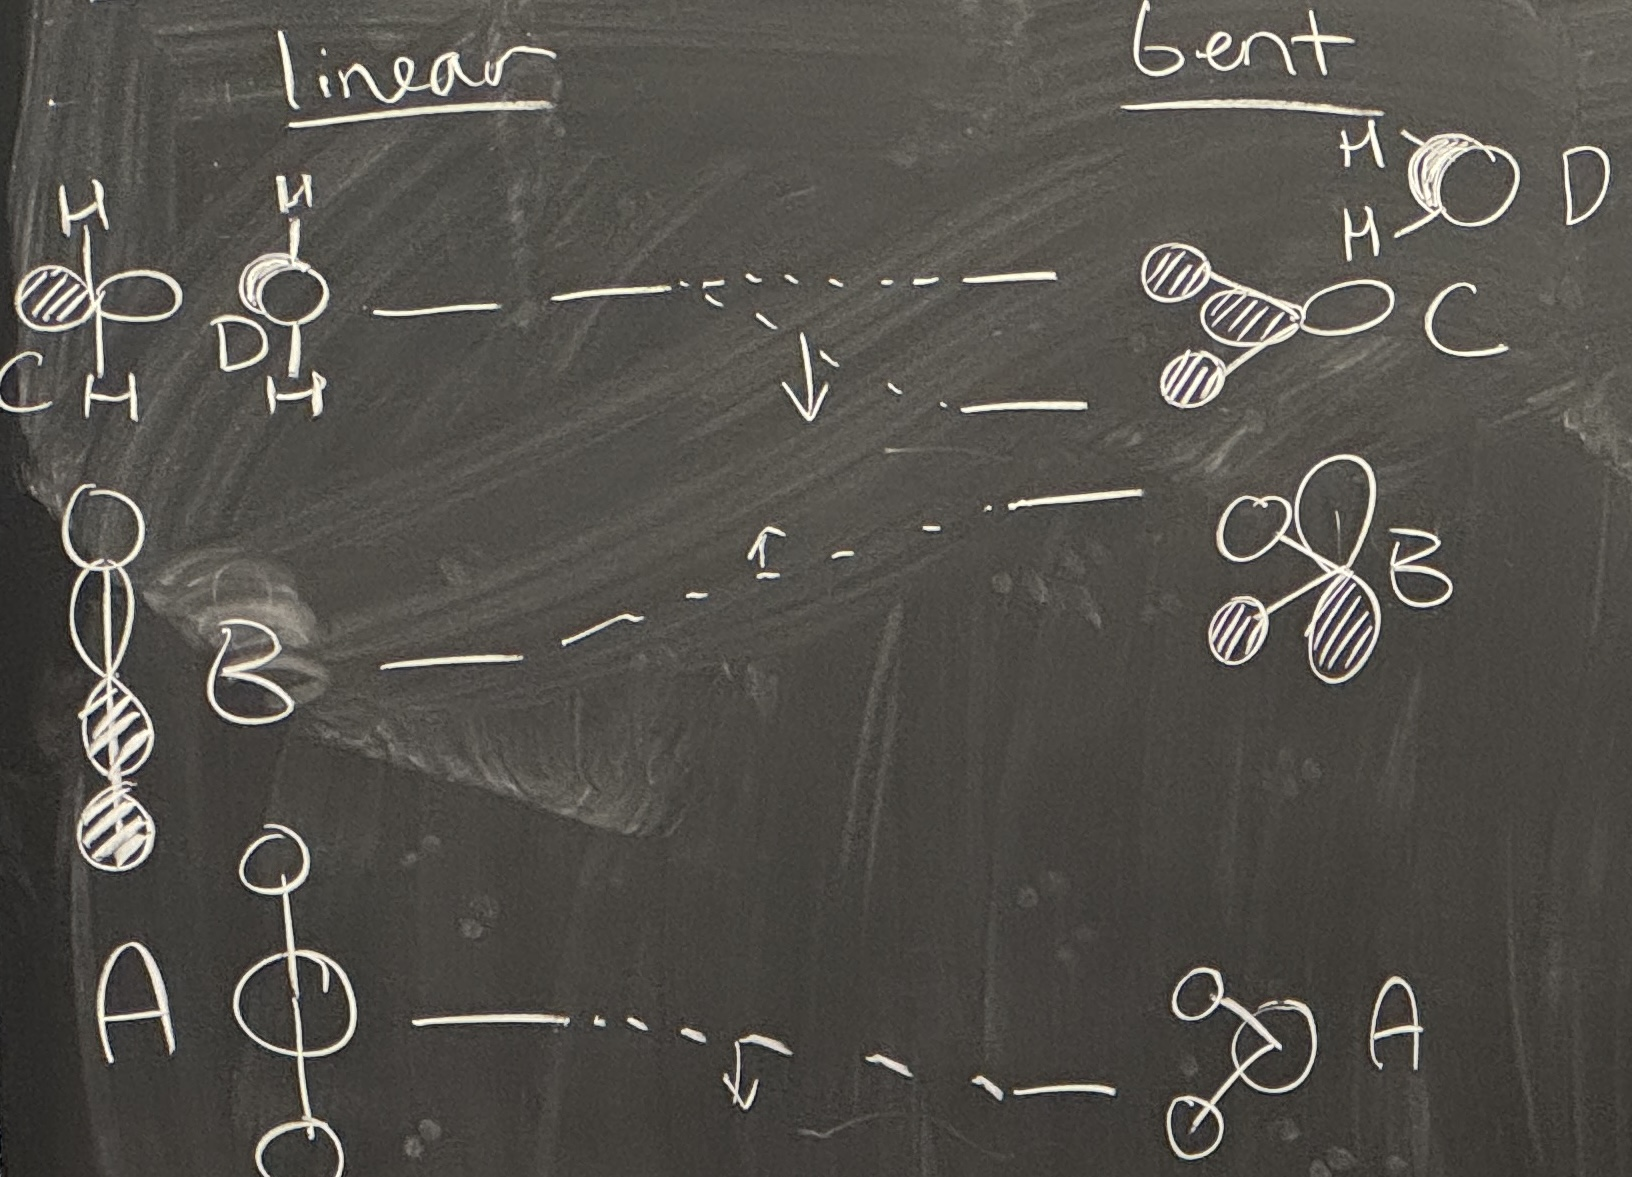
\includegraphics[width=0.4\linewidth]{QmotCH2.JPG}
        \caption{QMOT diagram for \ce{CH2}.}
        \label{fig:QmotCH2}
    \end{figure}
    \begin{itemize}
        \item Two geometries: Linear and bent.
        \item Linear.
        \begin{enumerate}[label={\textbf{\Alph*}.}]
            \item Linear chain of $s$-orbitals with matching phases.
            \item Linear chain of matching phases orbitals, with $p_x$ on carbon.
            \item One of the other $p$-orbitals, with no phasing.
            \item The last remaining $p$-orbital, again with no phasing.
        \end{enumerate}
        \item Bent.
        \begin{enumerate}[label={\textbf{\Alph*}.}]
            \item Goes down slightly. We kept primary, and added secondary.
            \item Losing primary overlap and gaining a destabilizing secondary interaction; higher $E$ like before.
            \item Adding \emph{significant} constructive interference. Biggest effect again!
            \item Staying the same; no bonding interactions to begin or end with. We don't consider secondary interactions when there's no density at all there.
        \end{enumerate}
        \item Example species.
        \begin{itemize}
            \item \ce{H2O}: 8 electrons, bent.
            \begin{itemize}
                \item Note that this model predicts that \ce{H2O} has nondegenerate lone pairs, which has been experimentally verified!
                \item Bulk water acts as if it has degenerate lone pairs. We can read \textcite{bib:Anslyn} about this, but otherwise, it's outside the scope of the class.
            \end{itemize}
            \pagebreak
            \item \ce{CH2} (a \textbf{carbene}): 6 electrons, a mix of linear and bent!
            \begin{itemize}
                \item We'll return to carbenes in a few weeks.
                \item We'll define \textbf{triplet} (2 electrons in different orbitals) and \textbf{singlet} (2 electrons in same orbital) carbenes later.
                \item Triplet is \ang{136}, and singlet is \ang{105}, so the triplet is more linear and the singlet is more bent! The triplet has reactivity more characteristic of the linear orbital picture, and the singlet has reactivity more characteristic of the bent orbital picture.
                \item The triplet is more favored by \SI[per-mode=symbol]{9}{\kilo\calorie\per\mole}
            \end{itemize}
        \end{itemize}
    \end{itemize}
    \item Example QMOT diagram: Formaldehyde.
    \begin{figure}[h!]
        \centering
        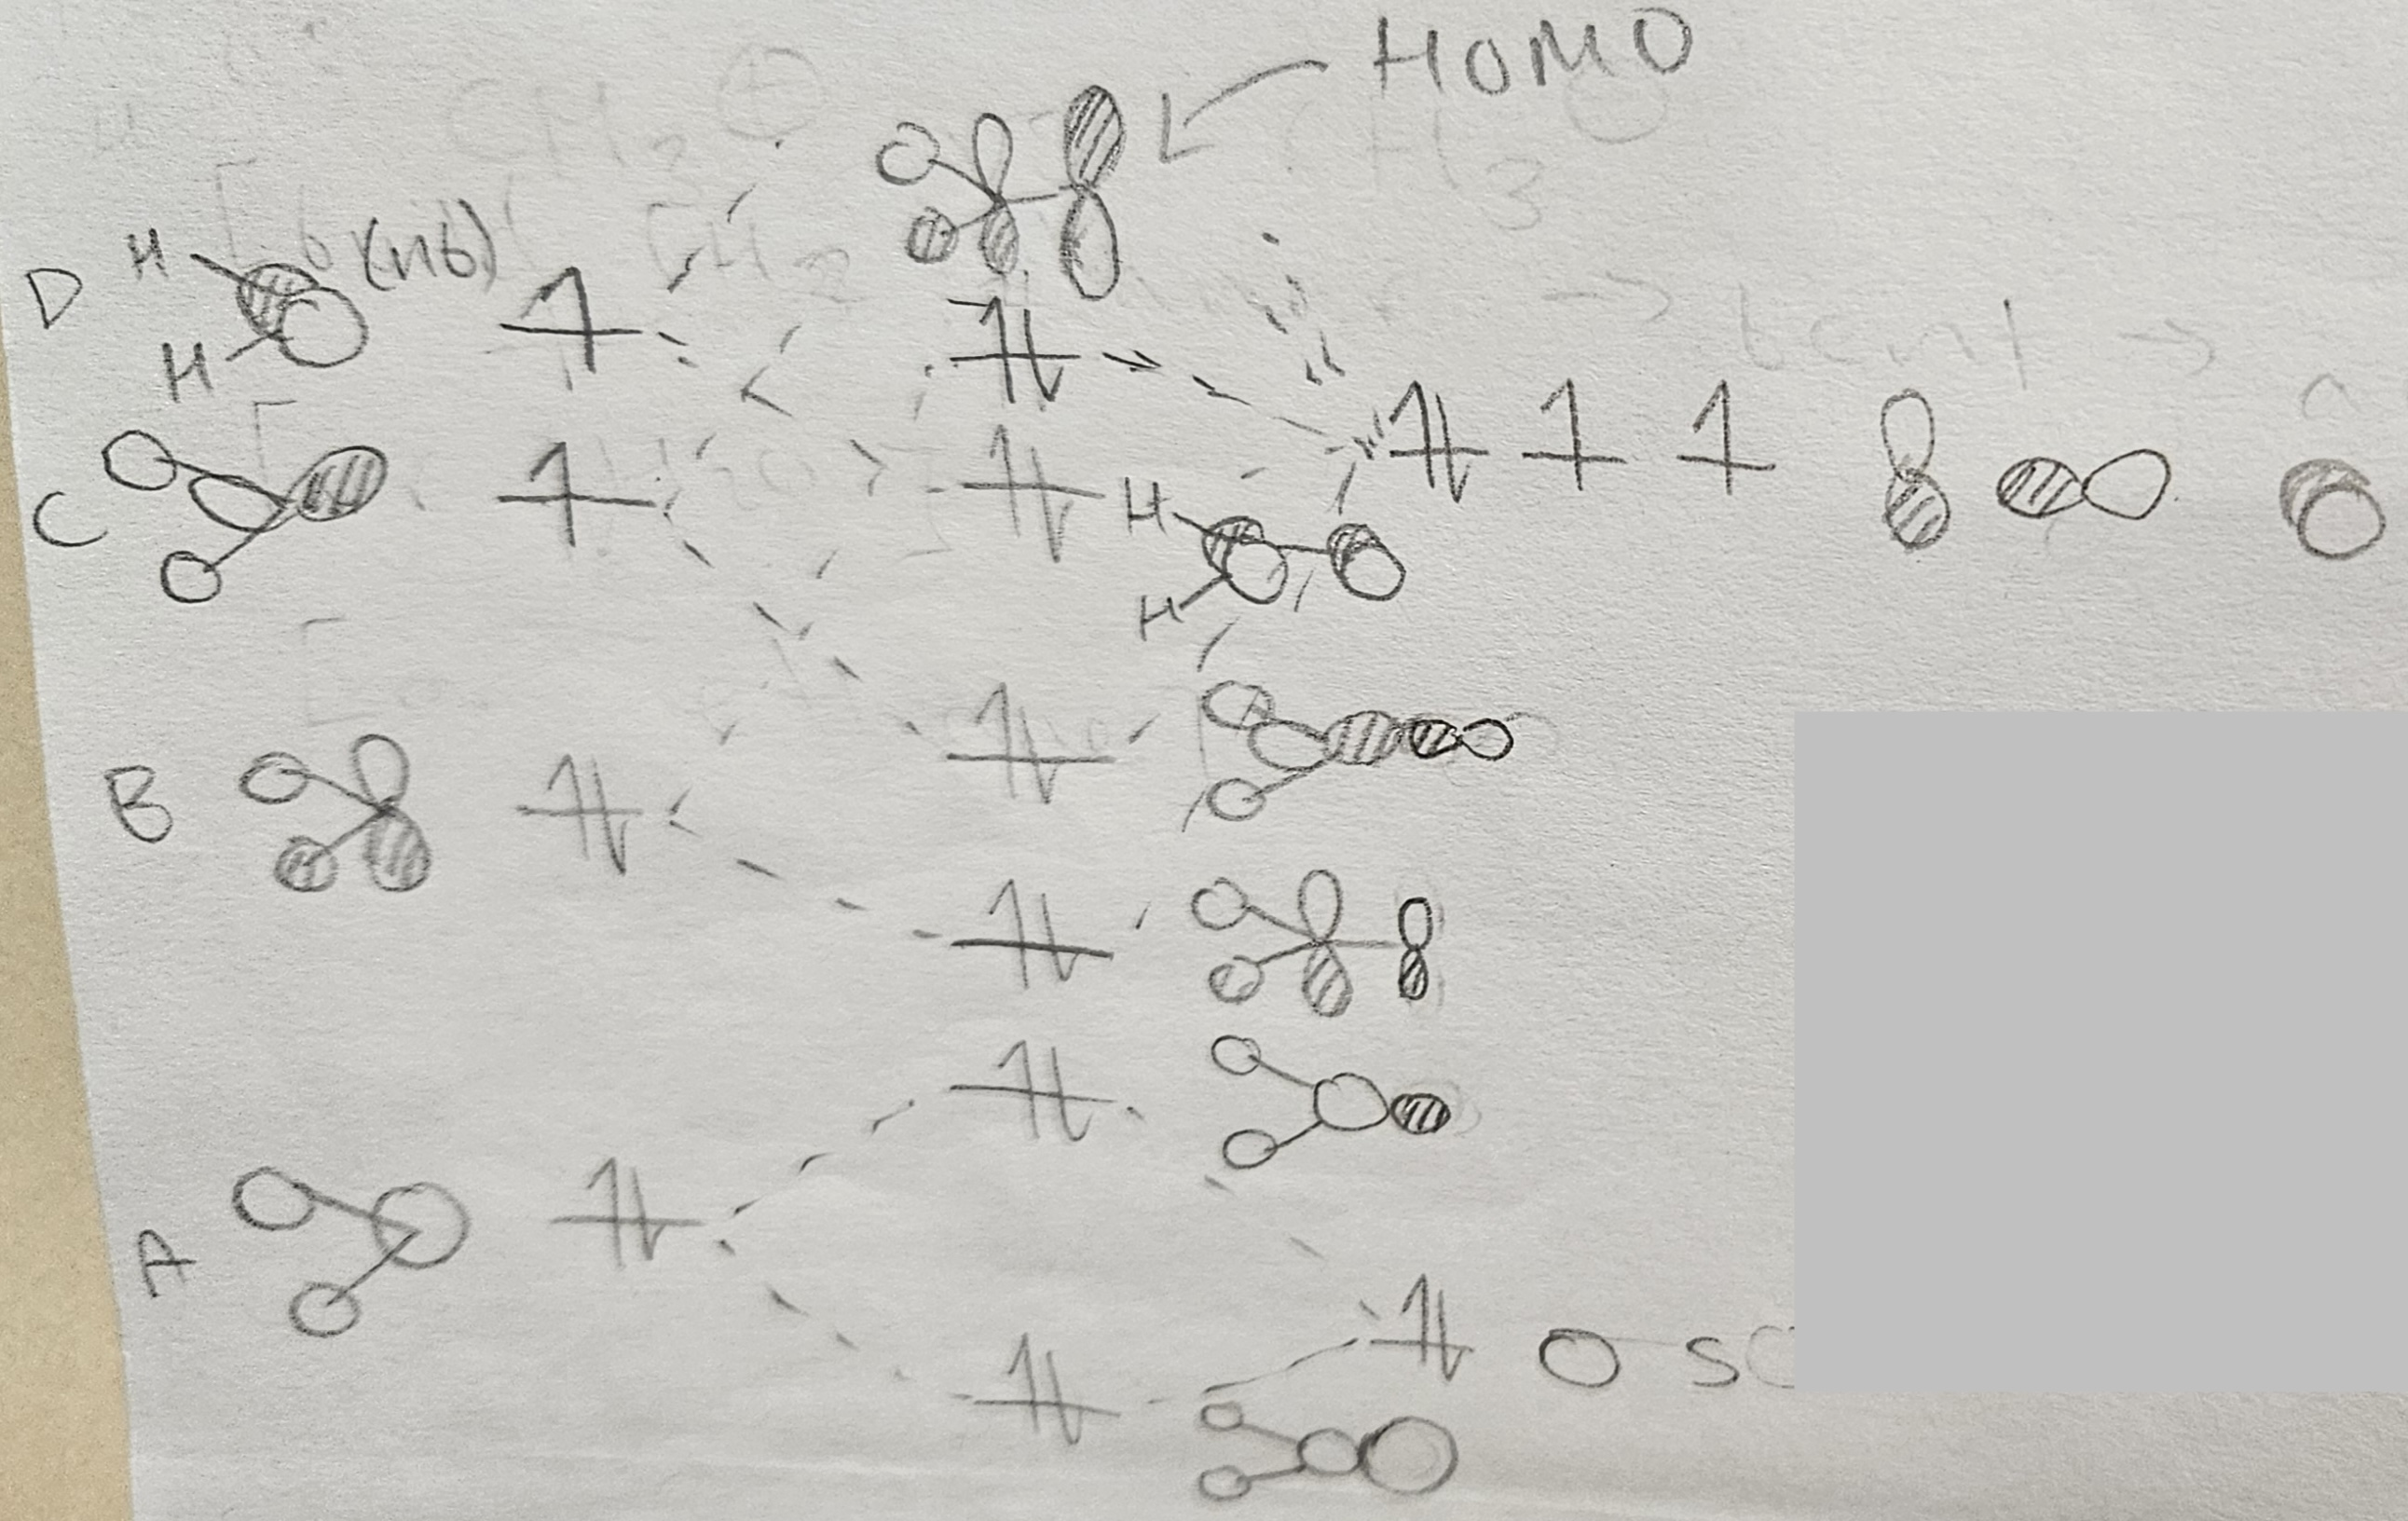
\includegraphics[width=0.6\linewidth]{QmotForm.jpg}
        \caption{QMOT diagram for formaldehyde.}
        \label{fig:QmotForm}
    \end{figure}
    \begin{itemize}
        \item The HOMO has a larger coefficient on \ce{O}; this explains why protonation occurs on \ce{O} and not \ce{C}!
    \end{itemize}
    \item Key takeaway: QMOT diagrams and MO diagrams both make the same predictions about the electronic structure and reactivity of formaldehyde (sanity check).
    \begin{itemize}
        \item Example: They both predict that carbonyls are nucleophilic on oxygen.
        \item Example: Orbital mixing is stronger when orbitals are of similar energy.
        \item Example: Orbital coefficients are larger on an atom when the MO is closer in energy to the AO that originates with that atom.
        \item Example: Orbitals are lower in energy on more electronegative atoms.
        \item Etc.
    \end{itemize}
\end{itemize}



\section{Bonding Models 2}
\begin{itemize}
    \item \marginnote{9/12:}Lecture 2 recap.
    \begin{itemize}
        \item QMOT for formaldehyde (see Figure \ref{fig:QmotForm}).
        \item Recall that the HOMO has a larger coefficient on oxygen, which means that protonation occurs on oxygen instead of carbon.
        \item No other topics from Lecture 2 are reviewed.
    \end{itemize}
    \item Today: Bonding models (continued).
    \pagebreak
    \item Lecture outline.
    \begin{itemize}
        \item Huckel theory.
        \item Aromaticity.
        \item Banana bonds.
        \item Wave functions.
    \end{itemize}
    \item \textbf{Huckel theory}: A quick way to build MOs for conjugated $\pi$-systems.
    \begin{itemize}
        \item Qualitatively great and quantitatively bad.
        \begin{itemize}
            \item Quick and dirty, but generates useful predictions.
            \item Not \emph{accurate}, but definitely \emph{useful}.
        \end{itemize}
        \item It is used to analyze the connectivity and topology of the $\pi$-system in a planar molecule.
        \item Key assumptions.
        \begin{itemize}
            \item The $\pi$-system is independent of the $\sigma$-network.
            \item You only consider valence electrons.
            \item Only neighboring orbitals interact, i.e., only $\pi$-orbitals on adjacent atoms.
            \item We ignore orbital overlap and electron repulsion.
        \end{itemize}
        \item These are some wild simplifications, but it is quick and useful!
        \item Rules.
        \begin{itemize}
            \item The number of $p$-AOs you mix equals the number of new MOs you make.
            \item The energy of the new MOs is distributed symmetrically around the \textbf{nonbonding energy level}.
            \item The number of nodes increases by 1 with each energy level.
            \item The MOs reflect the symmetry of the molecule.
        \end{itemize}
    \end{itemize}
    \item \textbf{Nonbonding energy level}: The energy of the nonbonding MOs in a Huckel diagram. \emph{Denoted by} $\bm{\alpha}$.
    \begin{itemize}
        \item This is also the energy of an electron in an empty $p$-AO.
    \end{itemize}
    \item Example Huckel diagram: Ethylene.
    \begin{figure}[h!]
        \centering
        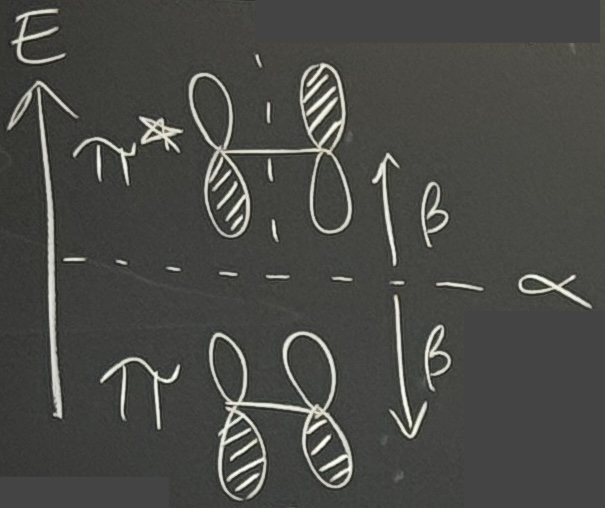
\includegraphics[width=0.18\linewidth]{HuckelEthylene.JPG}
        \caption{Huckel diagram for ethylene.}
        \label{fig:HuckelEthylene}
    \end{figure}
    \begin{itemize}
        \item Let's first confirm that this diagram meets all four Huckel theory rules.
        \begin{itemize}
            \item We get two new $\pi$-MOs from two $p$-AOs.
            \item The energy difference from the nonbonding energy level is called $\beta$.
            \item The number of nodes did increase from 0 to 1.
            \item The MOs are symmetric.
        \end{itemize}
        \item Thus, this is a valid Huckel diagram!
        \item Note: Do remember that symmetric splitting is \emph{not} accurate!
        \begin{itemize}
            \item On Tuesday, we (correctly) learned that destabilization energy $>$ stabilization energy.
        \end{itemize}
    \end{itemize}
    \item Example Huckel diagram: Allyl groups.
    \begin{figure}[H]
        \centering
        \begin{subfigure}[b]{0.4\linewidth}
            \centering
            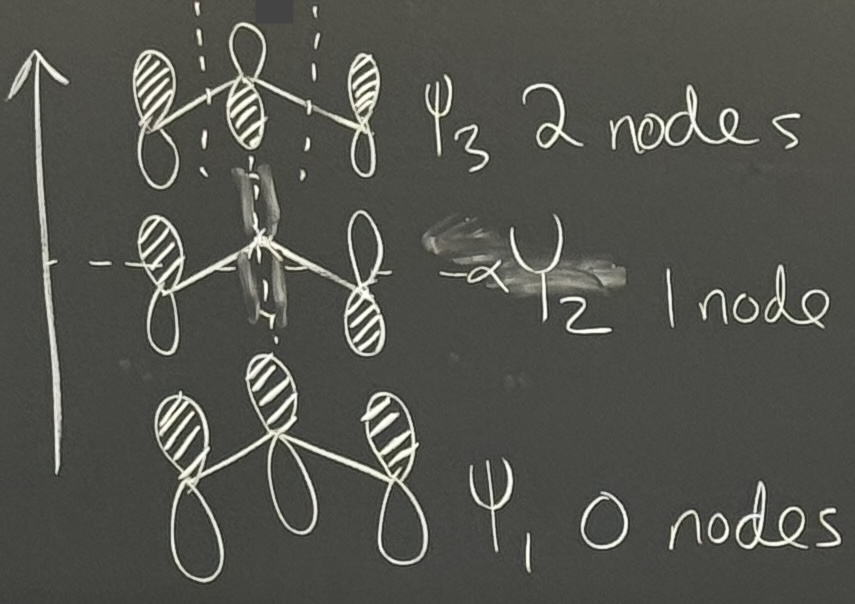
\includegraphics[width=0.685\linewidth]{HuckelAllyla.JPG}
            \caption{Diagram.}
            \label{fig:HuckelAllyla}
        \end{subfigure}
        \begin{subfigure}[b]{0.4\linewidth}
            \centering
            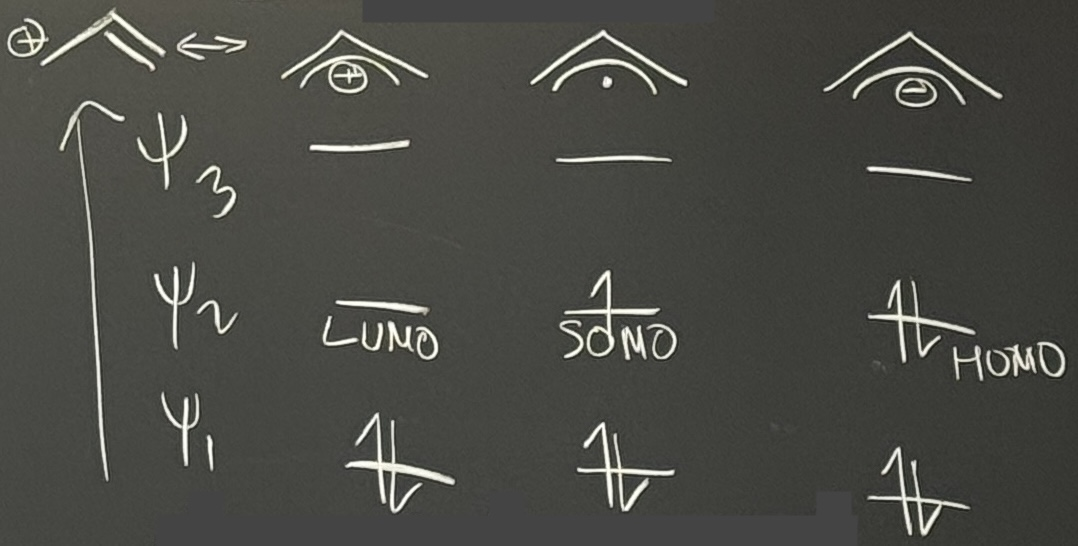
\includegraphics[width=0.95\linewidth]{HuckelAllylb.JPG}
            \caption{Filling orbitals.}
            \label{fig:HuckelAllylb}
        \end{subfigure}
        \caption{Huckel diagram for allyl groups.}
        \label{fig:HuckelAllyl}
    \end{figure}
    \begin{itemize}
        \item The lowest energy orbital is called $\psi_1$.
        \begin{itemize}
            \item It has 0 nodes.
        \end{itemize}
        \item The middle energy orbital is called $\psi_2$.
        \begin{itemize}
            \item To maintain symmetry, we have to delete the middle orbital and give opposite phases.
        \end{itemize}
        \item The highest energy orbital is called $\psi_3$.
        \begin{itemize}
            \item It has the 2 nodes we expect.
        \end{itemize}
        \item We now fill electrons for the allyl cation, radical, and anion (Figure \ref{fig:HuckelAllylb}).
        \begin{itemize}
            \item These species have 2, 3, and 4 electrons, respectively.
        \end{itemize}
        \item Now let's look at where each of these species will react.
        \begin{itemize}
            \item Nucleophiles will attack the LUMO of the cation.
            \item Radicals react with their SOMO (singly occupied molecular orbital).
            \item Electrophiles will engage the HOMO of the allyl anion.
        \end{itemize}
        \item But the LUMO, SOMO, HOMO are all $\psi_2$!
        \begin{itemize}
            \item $\psi_2$ has no density at the middle carbon, so all of these species should only react at the terminal carbons.
            \item This prediction of Huckel theory is experimentally confirmed!
            \item Intuitively, reacting at the terminals allows you to keep the double bond in play; thermodynamically, you wouldn't want to cleave it by reacting in the middle.
        \end{itemize}
    \end{itemize}
    \item Example Huckel diagram: Benzene.
    \begin{figure}[h!]
        \centering
        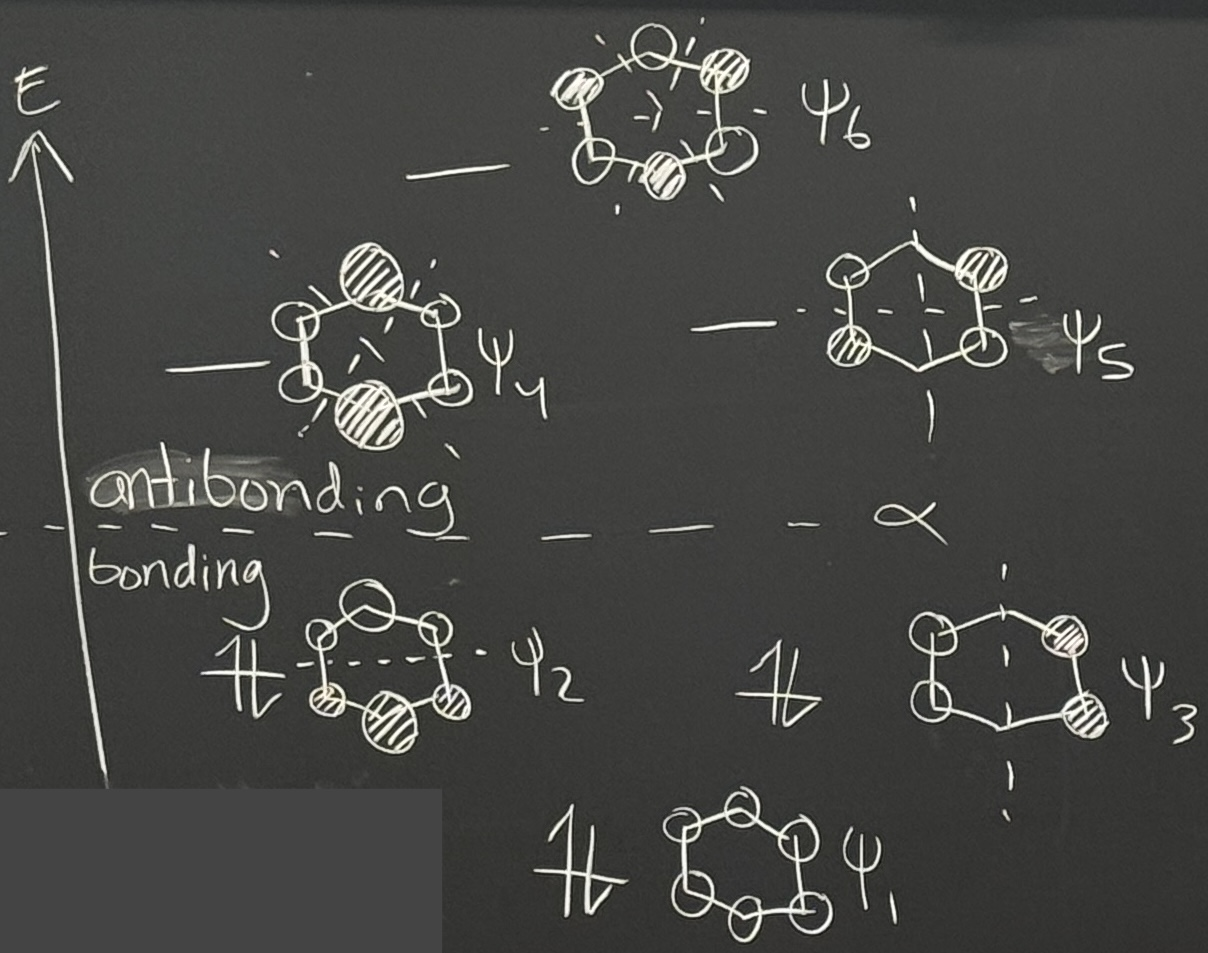
\includegraphics[width=0.4\linewidth]{HuckelBenzene.JPG}
        \caption{Huckel diagram for benzene.}
        \label{fig:HuckelBenzene}
    \end{figure}
    \begin{itemize}
        \item For cyclic systems, we draw a \textbf{Frost circle}.
        \begin{itemize}
            \item For benzene, the radius of the Frost circle is $2\beta$.
        \end{itemize}
        \item We create $\psi_1,\dots,\psi_6$.
        \begin{itemize}
            \item $\psi_2,\psi_3$ and $\psi_4,\psi_5$ are degenerate.
            \item No electron density on the central $p$-orbitals in $\psi_3$ implies bigger coefficients on the corresponding orbitals in $\psi_2$.
            \begin{itemize}
                \item See \textcite{bib:Anslyn} for more!!
            \end{itemize}
            \item $\psi_4,\psi_5$ have 2 nodes at angles.
            \item For $\psi_6$, we have 3 nodes through a hexagon, which is alternating shading.
        \end{itemize}
        \item $\alpha$ is the nonbonding level; higher is antibonding, lower is bonding.
        \item 6 electrons in benzene's bonding $\pi$-system yields stabilization.
        \begin{itemize}
            \item In particular, we observe stabilization relative to three ethylenes: An extra \SI[per-mode=symbol]{36}{\kilo\calorie\per\mole} of stabilization!
            \item Huckel theory can't really compare energy between two molecules; $\beta$ is more a qualitative parameter than a quantitative one.
        \end{itemize}
    \end{itemize}
    \item \textbf{Frost circle}: A circle in which we inscribe a regular $n$-gon with one point down --- where $n$ is equal to the number of carbons in the cyclic system --- that is used as a guide for drawing Huckel orbitals.
    \item Example Huckel diagram: Cyclobutadiene.
    \begin{figure}[h!]
        \centering
        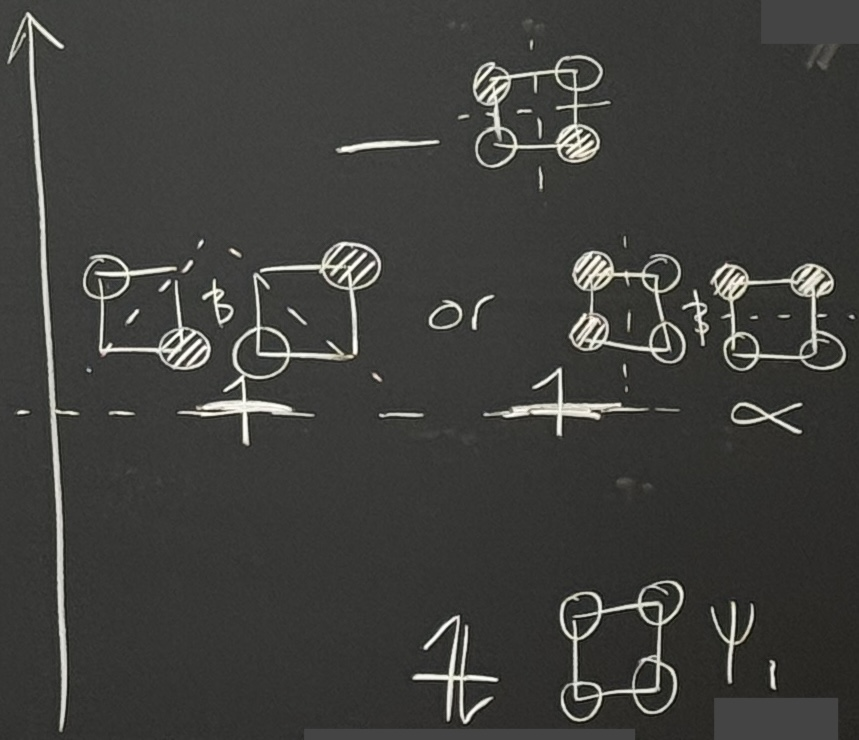
\includegraphics[width=0.25\linewidth]{HuckelCyclobutadiene.JPG}
        \caption{Huckel diagram for cyclobutadiene.}
        \label{fig:HuckelCyclobutadiene}
    \end{figure}
    \begin{itemize}
        \item $\psi_1$ has no phase inversion and no nodes.
        \item There are two different ways to draw the orbitals for $\psi_2,\psi_3$.
        \begin{itemize}
            \item We can dive deeper into this difference in \textcite{bib:Anslyn}.
        \end{itemize}
        \item No extra stability relative to three ethylenes!
        \item The model also predicts a ground-state triplet diradical.
        \begin{itemize}
            \item Indeed, this molecule is highly reactive and dimerizes spontaneously at \SI{35}{\kelvin}.
        \end{itemize}
    \end{itemize}
    \item We now do a deep dive into aromaticity.
    \item The history of aromaticity.
    \begin{itemize}
        \item In 1855, Hofmann (not Hoffmann) coins the term "aromatic" because these compounds were smelly.
        \item In 1861, we have Kekul\'{e}'s dream of a snake eating its tail.\footnote{"At least, Kekul\'{e} \emph{said} it was a dream!" - Masha. Good use of reasonable doubt and objectivity in her thinking!} This inspired a circle of electrons.
        \item In 1925, Robinson describes aromaticity as extra stabilization of a molecule.
        \item In 1931, Huckel puts forth \textbf{Huckel's rule}.
    \end{itemize}
    \item \textbf{Huckel's rule}: Cyclic, planar molecules with $4n+2$ continuous $\pi$-electrons are aromatic.
    \begin{itemize}
        \item If you have $4n$ electrons in a cyclic planar molecule with continuous $\pi$-electrons, then you are antiaromatic (extra unstable).
        \item Thus, these molecules usually distort out of the plane to break antiaromaticity and become nonaromatic.
        \begin{itemize}
            \item Both cyclobutadiene and cyclooctatetraene are antiaromatic. Cyclooctatetraene bends into a boat so that its $\pi$-orbitals are pointing toward each other.
        \end{itemize}
        \item No phase inversions are allowed; we must connect orbitals without crossing the $\sigma$-plane.
        \begin{itemize}
            \item What does this mean??
        \end{itemize}
    \end{itemize}
    \item Features of aromatic compounds.
    \begin{itemize}
        \item Aromatic stabilization energy (\SI[per-mode=symbol]{36}{\kilo\calorie\per\mole}).
        \item Equalization of the bond lengths.
        \begin{itemize}
            \item Essentially, the bond lengths do not alternate but rather share an identical bond order of 1.5.
        \end{itemize}
        \item Ring currents and magnetic properties.
        \begin{itemize}
            \item Those interested in polymer chemistry might be interested in exploiting these properties!
            \item Specifically, these are properties that come from a sea of electron density.
        \end{itemize}
        \item Benzene vs. hexa-1,3,5-triene.
        \begin{itemize}
            \item In benzene, all bond lengths are \SI{1.40}{\angstrom}.
            \item In hexa-1,3,5-triene, the single bonds are \SI{1.45}{\angstrom}, the terminal double bonds are \SI{1.34}{\angstrom}, and the internal double bond is \SI{1.37}{\angstrom}.
            \item The bond lengths of benzene equalize because benzene has two equally stable major resonance structures.
            \begin{itemize}
                \item This is why we often draw benzene as a hexagon with a circle in the middle: This is actually the most accurate picture of it!
            \end{itemize}
            \item The bond lengths of hexa-1,3,5-triene do \emph{not} equalize because the only resonance structure we can draw of it is a zwitterion, and thus will be a minor contributor.
        \end{itemize}
        \item Different kinds of reactivity.
        \begin{itemize}
            \item Example: Electrophilic aromatic substitution.
            \item This is very much distinct from alkene addition chemistry.
        \end{itemize}
    \end{itemize}
    \item \textbf{M\"{o}bius aromaticity}: Aromatic rings have one phase inversion (PI), like in a M\"{o}bius strip.
    \begin{figure}[h!]
        \centering
        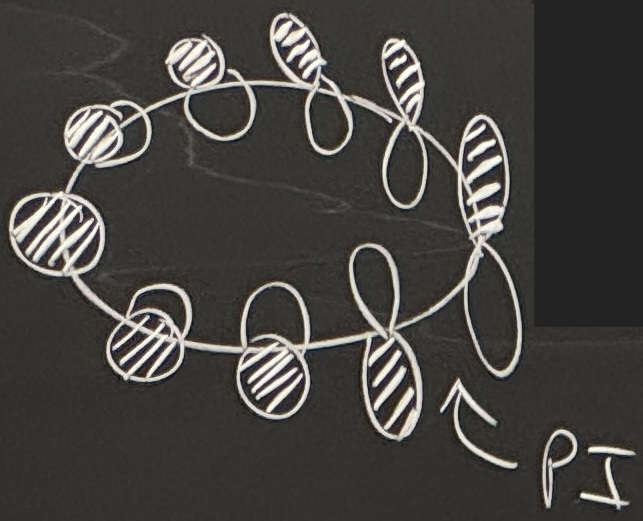
\includegraphics[width=0.18\linewidth]{MobiusAromaticity.JPG}
        \caption{M\"{o}bius aromaticity.}
        \label{fig:MobiusAromaticity}
    \end{figure}
    \begin{itemize}
        \item This is a different definition of aromaticity.
        \begin{itemize}
            \item We could research aromaticity for the rest of our lives if we wanted to.
            \item There's a whole field of research devoted to it, and we should look into it if we're interested!!
            \item A good starting point is \textcite{bib:MobAro}.
        \end{itemize}
        \item The single phase inversion is called a \textbf{M\"{o}bius topology}.
        \item Your PI happens at the sole node.
        \begin{itemize}
            \item This one node is allowed in M\"{o}bius aromaticity, but not in Huckel aromaticity
        \end{itemize}
        \item The M\"{o}bius topology predicts that compounds are aromatic if they have $4n$ electrons and antiaromatic if they have $4n+2$ electrons.
        \item To be clear, this content is outside the scope of this class, but Masha wants us to know about it and be able to research it if we so choose.
    \end{itemize}
    \item Ring current.
    \begin{figure}[h!]
        \centering
        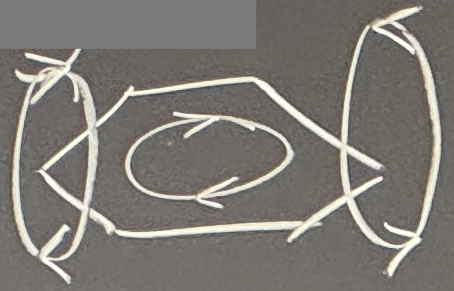
\includegraphics[width=0.12\linewidth]{RingCurrent.JPG}
        \caption{Ring current.}
        \label{fig:ringCurrent}
    \end{figure}
    \begin{itemize}
        \item Suppose you have an external magnetic field perpendicular to the $\sigma$-plane.
        \begin{itemize}
            \item This would induce the $\pi$-electrons to rotate through their MOs.
            \item These rotating electrons would then create an additional magnetic field.
            \item This new magnetic field would \emph{reinforce} the external magnetic field outside the aromatic ring and \emph{oppose} the external magnetic field inside the ring.
            \item The strength of the induced magnetic field is proportional to the current (i.e., the size of the ring).
        \end{itemize}
        \item Application (NMR): Ring protons are deshielded (higher $\delta$) outside and shielded (lower $\delta$) inside.
        \begin{itemize}
            \item Cyclohexene: No ring current, so we get a bit of downfield shift for the vinyl protons ($\delta$ 5.6).
            \item Benzene: Has a ring current, so we get a noticeable downfield shift ($\delta$ 7.3).
            \item\!\!\! [18]annulene: Has a large ring with many $\pi$-electrons, so we get a significant downfield shift for the external protons ($\delta$ 9.3) and a significant \emph{upfield} shift for the internal protons ($\delta$ $-2.9$).
        \end{itemize}
    \end{itemize}
    \item \textbf{Quadrupole}: Two dipoles aligned such that there is no net dipole.
    \begin{itemize}
        \item Example: The dipole aligned up and down in benzene --- perpendicular to the $\sigma$-plane of the molecule --- as opposed to (for instance) the linear dipole in fluoromethane.
        \item Lots of applications beyond the scope of this class, but we can look into it if we want.
    \end{itemize}
    \item \textbf{Banana bond}: A bent chemical bond that contains an unusually high concentration of $p$-character.
    \begin{itemize}
        \item The bent $p$-lobes of banana bonds look like bananas (see Figure \ref{fig:bananaBonds}), hence the name.
    \end{itemize}
    \item Example banana bonds: Cyclopropane.
    \begin{figure}[h!]
        \centering
        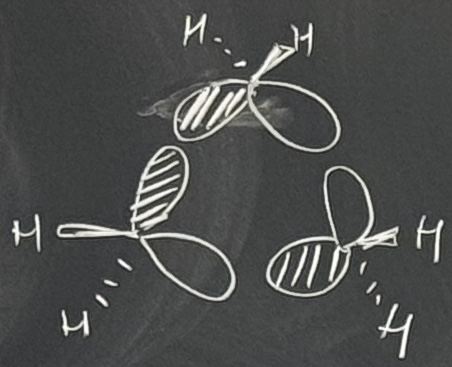
\includegraphics[width=0.17\linewidth]{bananaBonds.JPG}
        \caption{Banana bonds in cyclopropane.}
        \label{fig:bananaBonds}
    \end{figure}
    \begin{itemize}
        \item Cyclopropane needs more $p$-character because of its \ang{60} bond angles; $p$-character helps bonds bend.
        \begin{itemize}
            \item Specifically, the \ce{C-C} bonding orbitals in cyclopropane are $sp^5$-hybridized.
        \end{itemize}
        \item The excess of $p$-character in the \ce{C-C} bonds means that the \ce{C-H} bonds of cyclopropane have correspondingly more $s$-character.
        \begin{itemize}
            \item This makes the \ce{C-H} bonds in cyclopropane shorter than usual!
            \item Indeed, there is something of a "conservation" of bonding character: The $s$-character that's not in the $\sigma$-bonds has to go somewhere.
        \end{itemize}
        \item Group orbitals (HOMO) degenerate.
        \begin{itemize}
            \item The \textbf{Walsh orbitals} have more $\pi$-character, so cyclopropane is $sp^2$-like.
            \item This means it is a good $\pi$-donor and a bad $\pi$-acceptor.
            \item Example of donation: The dimethylcyclopropyl cation is very stable because all of the $sp^2$-character is getting donated into the carbocation's empty orbital. See Figure \ref{fig:HIAexc} for more.
        \end{itemize}
    \end{itemize}
    \item Wave functions.
    \begin{itemize}
        \item Review \textcite{bib:Anslyn}, Chapters 4 \& 14!!
        \begin{itemize}
            \item Also look up your Gen Chem or Quantum notes if it's been a while.
            \item Is there anything relevant to review in Chapter 4??
        \end{itemize}
        \item All bonding theories draw upon QM descriptions of electrons as waves existing in \textbf{orbitals}.
    \end{itemize}
    \item \textbf{Orbital}: A wave function that is a specific solution to the \textbf{Schr\"{o}dinger equation}.
    \begin{itemize}
        \item Masha draws the $1s,2s,3s$ orbital penetration graph, as well as what these orbitals look like.
        \item Recall that orbitals have \textbf{lobes} and \textbf{nodes}!
    \end{itemize}
    \item \textbf{Schr\"{o}dinger equation}: The following equation, where $E$ is the energy of the electron, $\psi$ is the wave function describing the position of the electron in space, and $H$ is the \textbf{Hamiltonian operator}. \emph{Given by}
    \begin{equation*}
        H\Psi = E\Psi
    \end{equation*}
    \begin{itemize}
        \item $\psi^2$ is the probability of finding an electron in a specific position (i.e., the electron density!).
        \item Big $\Psi$ is the total molecular wave function, and little $\psi$ is a molecular orbital.
    \end{itemize}
    \item \textbf{Hamiltonian operator}: A representation of all forces acting on the system, such as the kinetic energy of the electron and nucleus, nuclear-nuclear repulsion, electron-electron repulsion, etc.
    \item Next week, we'll talk about DFT and approximating solutions to the Schr\"{o}dinger equation. It will be like an intro to computational chemistry!
    \item Example: Electron density in \ce{H2} MOs.
    \begin{itemize}
        \item Masha redraws Figure \ref{fig:MOH2} to start, and Figure 7.3 from \textcite{bib:CHEM26100Notes}.
        \item The point is that\dots
        \begin{itemize}
            \item The bonding MO has a lot of electron density between the nuclei, even though you still have some at the atoms;
            \item The antibonding MO has minimal to no electron density between the nuclei; the AOs ($\phi_1^2,\phi_2^2$) are very separate.
        \end{itemize}
    \end{itemize}
\end{itemize}



\section{Chapter 1: Introduction to Structure and Models of Bonding}
\emph{From \textcite{bib:Anslyn}.}
\begin{itemize}
    \item \marginnote{9/23:}Good outline of the purpose of Chapter 1.
    \begin{itemize}
        \item Mostly along the lines of what we've talked about in class.
    \end{itemize}
    \item Why bother with simplistic bonding models if we can just compute everything quantum mechanically nowadays?
    \begin{itemize}
        \item "A string of computer-generated numbers is just no substitute for a well-developed feeling for the nature of bonding in organic molecules" \parencite[3]{bib:Anslyn}.
        \item "It is still true --- and will be true for some time --- that descriptive models of bonding that are readily applicable to a wide range of situations are the best way to attack complex problems" \parencite[4]{bib:Anslyn}.
    \end{itemize}
\end{itemize}


\subsection*{Section 1.1: A Review of Basic Bonding Concepts}
\begin{itemize}
    \item Vocab for Gen Chem-level quantum mechanics.
    \begin{itemize}
        \item Most of these I know without review.
    \end{itemize}
    \item \textbf{Spin paired} (electrons): Two electrons in the same orbital with opposite-signed $m_s$ values.
    \item \textbf{Correlation}: The ability of an electron to feel the trajectory of another electron and therefore alter its own course so as to minimize Coulombic repulsions and keep the energy of the system to a minimum.
    \item The strengths and weaknesses of Lewis structures.
    \begin{itemize}
        \item Pros: Predict the number of bonds an atom forms, whether it has lone pairs, and whether any double or triple bonds form.
        \item Cons: Does not describe the structure or reactivity of any given species.
    \end{itemize}
    \item Example: Why formal charge is much more a method of "bookkeeping" nowadays than anything accurate.
    \begin{itemize}
        \item In the tetramethylammonium cation, we put the formal positive charge on the nitrogen.
        \item However, computational studies show that since nitrogen is more electronegative than carbon, a $\delta^-$ rests on nitrogen in the actual structure, and every carbon shares \sfrac{1}{4} of the positive charge.
    \end{itemize}
    \item VSEPR's geometrically perfect bond angles are only observed in simple, symmetric molecules.
    \begin{itemize}
        \item However, words like "tetrahedral" and "trigonal" are broadly used to suggest an idea, even when they're not \emph{strictly} accurate.
    \end{itemize}
    \item VSEPR "is not based on any first principles analysis of electronic structure theory. It is a simple way to rationalize observed trends" \parencite[8]{bib:Anslyn}.
    \begin{itemize}
        \item Indeed, it is not clear that bonding orbitals or lone pairs really \emph{have} any well-defined notion of size.
        \item Note that singly occupied orbitals (e.g., radicals) do not have repulsive effects in VSEPR because they are able to bond to doubly occupied orbitals.
    \end{itemize}
    \item \textbf{Steric repulsion}: The buttressing of filled orbitals that cannot participate in bonding, where the negative electrostatic field of the electrons in the orbitals is repulsive.\footnote{Don't forget that Alison Wendlandt believes that this definition of sterics is fundamentally flawed, and that overlap is actually beneficial to a point!}
    \item \textbf{Hybridization}: The method of adding and subtracting atomic orbitals on the same atom.
    \begin{itemize}
        \item "Remember that orbitals are mathematical solutions to the Schr\"{o}dinger equation, and that the addition and subtraction of mathematical equations is just an exercise in algebra. It is a perfectly valid operation to add orbitals as long as one also does the corresponding subtraction" \parencite[9]{bib:Anslyn}.
        \begin{itemize}
            \item Someday, I should take linear combinations of $s$ and $p$ wave functions and confirm that they're still orthogonal and in the solution space of the Schr\"{o}dinger equation!!
        \end{itemize}
        \item It's called hybridization because we're literally forming \emph{hybrids} somewhere between the polar extremes of an $s$ and $p$ orbital!
        \item As with VSEPR bond angles, VBT hybridizations deviate from the $sp$, $sp^2$, or $sp^3$ ideal in most organic molecules, but we loosely retain these terms regardless to convey an idea.
    \end{itemize}
    \item \textcite{bib:Anslyn} goes over a cool connection between the hybridization index (as defined in class) and experimentally observed \ce{{}^1H}-\ce{{}^13C} NMR coupling.
    \item The localization of electrons in a chemical bond per VBT is exactly the impression of bonding that is given by a Lewis structure!
    \item Some useful content on polar covalent bonding that is slightly beyond the scope of the class.
    \begin{itemize}
        \item "Introducing polarity into a bond strengthens it" \parencite[12]{bib:Anslyn}.
        \item Pauling electronegativity is based on the BDEs of molecules, while Mulliken electronegativity is based on the IEs of atoms.
        \begin{itemize}
            \item Additional electronegativity scales by Nagle, Allen, Sanderson, Allred-Rochow, Gordy, Yuan, and Parr.
            \item Takeaway: Electronegativity is a hard concept to put your finger on!
        \end{itemize}
        \item The real use of electronegativity is in comparing \emph{relative} electronegativities, and all scales more or less agree here.
    \end{itemize}
    \item \textbf{Field effect}: The withdrawing of electron density through space, rather than through $\sigma$-bonds.
    \item Additional irrelevant content.
    \item Application of quadrupoles: Proving that $sp^2$-\ce{C} is more electronegative than \ce{H}.
    \item \textbf{Resonance energy}: The energy of stabilization imparted by resonance. \emph{Also known as} \textbf{delocalization energy}.
    \item Why is delocalization stabilizing from the point of view of quantum mechanics?
    \begin{itemize}
        \item Recall that in the particle in a box, the energy levels are given by
        \begin{equation*}
            E_n = \frac{n^2h^2}{8mL^2}
        \end{equation*}
        \item As $L$ increases (i.e., as we expand the box/delocalize), the energy goes down.
    \end{itemize}
    \item Lots more on resonance.
\end{itemize}


\subsection*{Section 1.2: A More Modern Theory of Organic Bonding}
\begin{itemize}
    \item Molecular orbital theory has the same predictive power as the models in Section 1.1 (Lewis structures, VSEPR, and VBT), but it can better explain certain structural issues and experimental observations, too.
    \begin{itemize}
        \item MO theory extracts certain key concepts and trends that result from the output of quantum mechanical calculations to lead to a more rigorous, descriptive model of organic bonding than Lewis structures, VSEPR, and VBT can.
    \end{itemize}
    \item VBT and MO theory are often fairly interconvertable mathematically!
    \begin{itemize}
        \item Thus, it is \emph{not} necessarily true that MO theory is "better" than VBT.
        \item Rather, both models (and any combination thereof) are approximations of the true answer --- a full solution to the Schr\"{o}dinger equation.
    \end{itemize}
    \item A more detailed analysis of the QMOT examples from class; definitely worth returning to!!
\end{itemize}


\subsection*{Section 1.3: Orbital Mixing --- Building Larger Molecules}
\begin{itemize}
    \item Goes over the mixing of fragments/group orbitals in detail. Relevant to PSet 1!!
    \item The later sections would likely be quite useful for my development as a chemist, but probably aren't immediately relevant to this course.
\end{itemize}



\section{Chapter 14: Advanced Concepts in Electronic Structure Theory}
\emph{From \textcite{bib:Anslyn}.}
\subsection*{Section 14.1: Introductory Quantum Mechanics}
\begin{itemize}
    \item Some basic and some more advanced quantum mechanics, but all stuff with which I am eminently familiar from my undergrad coursework.
\end{itemize}


\subsection*{Section 14.3: A Brief Overview of the Implementation and Results of HMOT}
\begin{itemize}
    \item \textbf{HMOT}: Huckel molecular orbital theory.
    \item A much more mathematical treatment of Huckel theory, similar to what I saw in CHEM 26100. It does rationalize the benzene coefficients, though, so probably worth returning to!!
\end{itemize}


\subsection*{Section 14.5: Some Topics in Organic Chemistry for Which Molecular Orbital Theory Lends Important Insights}
\begin{itemize}
    \item More mathematics of aromaticity, cycles, etc. Probably a bit less useful.
\end{itemize}




\end{document}